\documentclass{standalone}
\usepackage{standalone}

\begin{document}
\chapter{Background Study}


\section{Historical View}
As far as we know that ANPR system was first invented in 1976. It was done by the Police Scientific Development Branch in the UK. Industrial usage begun in 1979. But ANPR got more known in the 1990's for their cheap implementation from the previous costly systems. The first ANPR dataset was made in early 2000s. This system was used to solve a murder occurred in November 2005, in Bradford, UK, to locate and find the culprits behind the killing of Sharon Beshenivsky.

From that point forward tag acknowledgment has advanced and been utilized by police and different associations for various purposes and has turned out to be less expensive and speedier, yet not sufficiently shoddy for private utilize. In the following areas, a portion of the current techniques in the zone of tag location and acknowledgment will be talked about.

\section{Standard Bangla license plate}
\subsection{Vehicle types}
Vehicles are of different types in Bangladesh. As a result license plates don't stay at the same place for each vehicle.
Vehicles considered in this thesis work are - private car, bus, cng auto-rickshaw, truck. Though there were no previous format and standardization of the license plate in the past, currently government has enforced digital license plate for all vehicles which makes it a new case to handle and less error prone than the previous systems.

\subsection{Structure of the plate}
The digital Bengali license plate is normally written in two lines.

    \begin{figure}[ht]
    \centering
    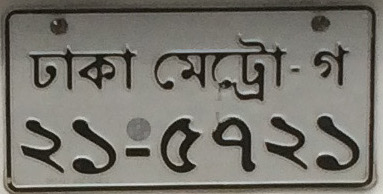
\includegraphics[scale=0.8]{./img/sample_plate}
    \caption{Example of a digital license plate in Bangla}
	\label{fig:EX}
    \end{figure}

\par
As the example given the line on the top written in Bangla and the bottom line has all digits in Bangla.    

\subsection{Parts of plate number}
The top line got two parts. First part before the '-' denotes the city of the car license and then the second part denotes the series it is in.

The bottom line is the number of the license assigned to the particular vehicle by the licensing rules and regulation of Bangladesh Road Transport Authority.

	\begin{figure}[ht]
    \centering
    
\includegraphics[scale=0.8]{./img/up}
    \caption{upper portion of license plate}
	\label{fig:UP}
    
    
\includegraphics[scale=0.8]{./img/down}
    \caption{bottom part of license plate}
	\label{fig:DOWN}
    
    \end{figure} 
\subsection{Plate fonts}
Digital license plate is offering verified fonts, but in Bangladesh those rules are not strictly followed by all vehicle owners. Also the current dataset doesn't have any universal font. So, the fonts can be different but easily understandable for this thesis work.


\section{Literature Review}
The first task was to find the problem domain to work on. The next task was to make literature reviews for our work plan and also for ensuring that we are not doing something again or worse. We've found few papers related to ALPR for Bengali languages and many more in different languages. Finally, we did select 24 papers to read and review for our thesis work. We've written 7 review papers those seemed close to our topic. From those papers and reviews we've managed to find and understand our particular domain of work which will be described in the later parts.

  \section{Related Works}
The rest of the chapter will discuss some of the previous works related to license plate recognition.The whole task is divided into five main steps: Preprocessing, Feature analysis, Region analysis, Character segmentation, Recognition.
	
\begin{figure}
    \centering
    \includegraphics[scale=1.0]{./img/steps}
    \caption{Steps of ALPR system}
    \label{fig:STEPS}
\end{figure} 
    
These steps are going to be discussed briefly in this chapter.

  \documentclass{standalone}
\usepackage{standalone}

\begin{document}

\section{Preprocessing}

Preprocessing techniques are used to get a better performance in the next sections. This is one of the key task after image acquisition. It ensures good data input for the main parts of the license plate detection and recognition system.

Most common approach is done in two steps. The image is converted to a gray scale image format to the next steps (Waterhouse-2006) \cite{waterhouse-2006}. Then, any additional noise is reduced from the image with different types of algorithms in different cases. Most common techniques for reducing noise from input image are the Median filter(Songke and Yixian-2011) \cite{songke-yixian}
and Gaussian filter(Sedighi and Vafadust 2011) \cite{sedighi-vafadust}. Contrast enhancement is an additional technique followed by many researchers(Abolghasemi and Ahmadyfard - 2009) \cite{Abolghasemi2009} in this pre-processing part.

\end{document}
  \section{Feature Analysis}

For detecting the license plate, feature analysis must be done after an image is preprocessed properly.
Checking the edges for detecting any rectangle shaped area is the most common technique for feature analysis.
To detect the plate boundary, some researchers use horizontal lines and others look for vertical lines.
Edge detection is commonly done with Canny (Kong, Liu, Lu, and Zhou-2005) \cite{Kong2005}  and Sobel edge detection (Jiao, Ye, and Huang 2009 \cite{jiao_ye_huang_2009}).
As foe some exception some researches do not use edge detection, but try to find high contrast area (Huang, Chang, Chen, and Sandnes-2008) \cite{HUANG2008}. The theory behind this technique is - plates generally have higher contrast area than other parts of the image.
  \section{Region Analysis}

When the feature analysis is done, it is possible that several regions of the image can be candidates for the license plate portion. For solving this problem some filtering is needed to lower the number of candidates by analyzing and removing them. A very common technique to do the task is to consider features of the bounding rectangle of candidate region. For example we can consider - aspect ratio, size width, height and location for candidate filtering. For example, calculating the rectangles features for determining the license plate probable region is a common trick (Yoon,
Lee, and Lee - 2009) \cite{yoon_lee_lee_2009}. Also, Abolghasemi and Ahmadyfard (2009) \cite{abolghasemi_ahmadyfard_2009}, Tsai, Wu,
Hsieh, and Chen (2009) \cite{Tsai2009} and Kong et al. (2005) \cite{Kong2005} used some geometrical features of the candidate
regions to detect the actual plate region. Following this with
further addition of techniques Gazcón, Chesñevar, and Castro (2012) \cite{gazcon2012automatic} proposed that if the region can be divided into well defined siz sub sections then it is the license plate region. Other researches like Hung and Hsieh (2010) \cite{hsieh2009real} used geometrical features technique
with a more or less the same technique by considering characters into
of the number plate while filtering the candidate regions. A slightly different approach for determining the license plate region was proposed by Chen, Chen, Huang, and Wang
(2011) \cite{chen2011license} by using the high density edges followed by horizontal projection.

  \section{Character Segmentation}

For recognition of the characters sometimes it is needed to segment them before sending them to the recognition system. Different research used different techniques for this part of work.

Using histogram to segment the characters is a common trick first used by Songke and Yixian (2011) and Huang et al. (2008). The technique was to use the accumulation or summation of the vertical and horizontal projections. Connected-component labeling algorithm can be used for the purpose of character segmentation which was used by Yoon et al. (2009) and Maglad (2012). The algorithm acts in two steps. Detection of the connected characters those are in black while the background is white. Then labeling those character blobs with bounding box. This technique was implemented by Liaqat (2011) using two algorithms, Canny for detecting the edges then contour finding algorithm to find the connected edges. Labeling and segmentation can be done using other methods. Next recognition step used many of the information gained in this step. All these information can be passed to a method for recognizing characters. Tsai et al. (2009) tried further judgement of this step to ensure that the selected characters makes the actual license plate, not some other part of the image. The conditions to pass this test were that the width, and height of character rectangles must be similar, character density should be in a range, and the width must be less than the height.
  \section{Character Recignition}

For licesnse plate recognition there are few ways to complete the character recigntion part. The most common technique can be divided into two steps. At first, the characters from the previous step are provided to a recognition engine that can be coded or used as a package. For example, Open source Tesseract OCR is a great choice for character recognition engine. It generates text output from the given image of characters if it is well trained. In the second approach is to implement bespoke recognition methods. For each individual character, features are computed. For recognizing the characters, OCR system will extract features first, then compare them against patterns that have been implemented earlier (Juntanasub and Sureerattanan - 2005). Alginahi (2011) tried  to extract 88 features for each character following the same approach, then compared these features with previously extracted features. Songke and Yixian (2011) used histogram to extract characters and template matching for recognition. Later when the neural network techniques got famous, Ghosh, Sharma, Islam, Biswas, and Akter - 2011 used them for character recognition. The module is trained first and then used for recognizing characters using the previously given taining feature dataset.
  \section{Comparisons}

The accuracy of license plate recognition system can be described in three parts - license plate detection, character recogntion, overall accuracy. Table \ref{tab:comparison} gives an overview related to the approach and problems of some previous research work.

\begin{table}[htb]
	\centering
	\begin{tabular}{|l|c|c|c|}
		\hline
		\multicolumn{1}{|c|}{Author and year}
		& \multicolumn{1}{|c|}{Detection (\%)}
		& \multicolumn{1}{|c|}{Recogntion (\%)} 
		& \multicolumn{1}{|c|}{Overall (\%)} \\ 
		\hline
		    
		Kong et al. (2005)\cite{Kong2005} & 96.1 &  & \\ \hline
		Juntanasub and Sureerattanan (2005) \cite{juntanasub2005car} & 92  &  & \\ \hline
		Waterhouse (2006)\cite{waterhouse-2006} & 96 & 83 and 93 & \\ \hline
		Huang, Chen, Chang, and Sandnes (2009)\cite{hsieh2009real} & 96.7 & 97.1  & 93.9 \\ \hline
		Alginahi (2011)\cite{alginahi2011automatic} & 98.3 & 98.63 & 94.9 \\ \hline
		Maglad (2012)\cite{maglad2012vehicle} & 95 & 91 & \\ \hline
		Joarder, Mahmud, Tasnuva, Kawser, Bulbul (2012)\cite{joarder2012bangla} & 92.1 & 84.16 & 75.51 \\ \hline
	\end{tabular}
	\caption{Comparison Table}
	\label{tab:comparison}
\end{table}




  
  
\section{Summary}
Review of previous works shows that the edge detection approach can be used effectively to find the license plate region. Geometrical feature analysis is an appropriate approach for this. Some researches used their own recogntion system, others used OCR engines like - teserract. Some parts of all these research can be used further in this work, others are of no use for future work.

\end{document}